\documentclass[lm-default]{l3doc}
\usepackage[scale=10pt]{char2path}
\usepackage{listings, hyperref}
\lstset{basicstyle = \footnotesize\ttfamily, numbers = left}

\usepackage[mono = false]{libertine}
\AddToHook{env/function/before}{\vspace*{-.7\baselineskip}}
\AddToHook{env/syntax/after}   {\par\vspace*{.2\baselineskip}}
\makeatletter
\def \@key  #1{\textcolor{red}{\textbf{\texttt{#1}}}\:\texttt{=}\:}
\def \s@key #1{\textcolor{red}{\textbf{\texttt{#1}}}}
\DeclareDocumentCommand \key s {\IfBooleanTF{#1}\s@key\@key}
\DeclareCommandCopy \val \meta
\def \TFF {true\textup{\textbar\textbf{false}}}
\def \TTF {\textup{\textbf{true}\textbar}false}
\def \HoLogo@ApLaTeX #1{^^A
  \HOLOGO@mbox {A\kern -.05em p\kern -.05em \hologo{LaTeX}}}
\newcounter{example}[subsection]
\renewcommand\theexample{\thesubsection.\arabic{example}}
\newwrite\example@out
\def\example@name{\jobname.example.aux}
\long\def\example@start{\begingroup\@bsphack
  \immediate\openout\example@out=\example@name
  \let\do\@makeother\dospecials\catcode`\^^M\active
  \def\verbatim@processline{\immediate\write\example@out{\the\verbatim@line}}^^A
  \verbatim@start}
\long\def\example@end{\immediate\closeout\example@out\@esphack\endgroup
  \trivlist\item[]\relax
    \leavevmode\hbox to \z@{^^A
      \hbox to \z@{\hss{\footnotesize[\theexample]}\hskip4pt}
      \begin{minipage}[c]{.72\textwidth}^^A
        \small\verbatiminput \example@name^^A
      \end{minipage}^^A
      \fbox{^^A
        \begin{minipage}[c]{.26\textwidth}^^A
          \normalsize\input \example@name^^A
        \end{minipage}^^A
      }^^A
    \hss}^^A
  \endtrivlist}
\newenvironment{example}
  {\stepcounter{example}\example@start}{\example@end}
\makeatother
\newlist{keyval}{itemize}{10}
\setlist[keyval]{leftmargin = 0pt, labelsep = 0pt}
\makeindex

\title{^^A
  The \pkg{char2path} Package\thanks{^^A
    \url{https://github.com/zongpingding/char2path},
    \texttt{https://ctan.org/pkg/char2path}^^A
  }^^A
}
\author{^^A
  Eureka\thanks{^^A
    \href{mailto:<email>@<domain>}{\texttt{<email>@<domain>}}},~
  Mingyu Xia\thanks{^^A
    \href{mailto:xiamingyu@westlake.edu.cn}{\texttt{xiamingyu@westlake.edu.cn}}^^A
  }^^A
}
\date{Released 2025-08-01\quad \texttt{v1.0.0}}

\begin{document}

\maketitle

\begin{documentation}

\section{Introduction}

The \pkg{char2path} package (conducted with \LaTeX3) provides
a \LaTeX\ package that converts characters into Ti\textit k\/Z paths.
It supports various compilation methods, such as \hologo{pdfLaTeX},
\hologo{XeLaTeX}, \hologo{ApLaTeX} (pending for check), \hologo{LuaLaTeX}, etc.

\section{Usage}

To load this package, write the line
\begin{quote}
  |\usepackage[scale = |\meta{int}|pt]{char2path}|
\end{quote}

Here, the integral number \meta{int} supports the following choices,
and the converted paths will be scaled to the corresponding factors.

\begin{center}
  \begin{tabular}{*9c}
    \toprule
    Pound   & |10pt|  & |11pt|  & |12pt|  &
    |13pt|  & |14pt|  & |15pt|  & |16pt|  & (Pending...)\\
    \midrule
    Factor  & |0.820| & |0.902| & |0.984| &
    |1.066| & |1.148| & |1.230| & |1.311| & ...\\
    \bottomrule
  \end{tabular}
\end{center}

\begin{function}{\chartopath}
  \begin{syntax}
    \cs{chartopath} \oarg{key-vals} \marg{string}
  \end{syntax}
  The mandatory argument accepts the required input string, and the optional
  argument accepts the following keys to set the style how the string converts
  to path.
  \begin{keyval}
    \item [\key{draw, fill}] \val{color} can set the color of the outline/fill of string
    (Default: |black|).
    \item [\key{outline}] \val{dim} can set the outline of the string
    (Default: |1|).
    \item [\key{scale}] \val{fp num} can set the scale of the string
    (Default: |1|).
    \item [\key{fading}] \val{clist} can set the two colors and one direction for fading the whole string.
  \end{keyval}
\end{function}

\section{Examples}

This package can convert the following characters to path by default:
including \textrm{Latin Modern Roman},
\textrm{Latin Modern Sans} (will be supported soon)
and \texttt{Latin Modern Mono}.

\DeleteShortVerb\| \DeleteShortVerb\" \catcode`\^11\relax
\begin{center}
  \begin{minipage}[t]{.48\linewidth}
    \fbox{\hskip16pt\parbox[c][4\baselineskip]{\linewidth-24pt}{
      \chartopath{lmm}{!\#\ctpdollar"\%\&'()*+,-./012345678}\par
      \chartopath{lmm}{9:;<=>?@ABCDEFGHIJKLMNOP}\par
      \chartopath{lmm}{QRSTUVWXYZ[\ctpbackslash]^_`abcdefgh}\par
      \chartopath{lmm}{ijklmnopqrstuvwxyz\{|\}\ctptilde}\par
    }}
  \end{minipage}
  \hspace*\fill
  \begin{minipage}[t]{.48\linewidth}
    \fbox{\hskip16pt\parbox[c][4\baselineskip]{\linewidth-24pt}{
      \chartopath{lmr}{!\#\ctpdollar"\%\&'()*+,-./012345678}\par
      \chartopath{lmr}{9:;<=>?@ABCDEFGHIJKLMNOP}\par
      \chartopath{lmr}{QRSTUVWXYZ[\ctpbackslash]^_`abcdefgh}\par
      \chartopath{lmr}{ijklmnopqrstuvwxyz\{|\}\ctptilde}\par
    }}
  \end{minipage}
\end{center}
\MakeShortVerb\| \MakeShortVerb\" \catcode`\^7\relax

\subsection{Basic usage}

\noindent
\def\0{0123456789ABCabc./*}
The basic usage only print the outline of the inputted string.
\begin{example}
  \chartopath{lmm}\0
\end{example}
\noindent
Users can pecific the color of outline and fill,
or specific the scale of inputted characters.
Just like the keys in \pkg{Ti\textit k\/Z}
\begin{example}
  \chartopath[draw = none, fill = blue]{lmm}\0
\end{example}

\begin{example}
  \chartopath[draw = blue, fill = red, scale = 1.2]{lmm}\0
\end{example}

Fading is also supported

\begin{example}
  \chartopath[fading = {red, green, horizontal}]
    {lmm} {0123456789ABCabc./*}
\end{example}

\begin{example}
  \chartopath[fading = {blue, violet, horizontal}]{lmm}\0
\end{example}

\begin{example}
  \chartopath[fading = {teal, violet, vertical}]{lmm}\0
\end{example}

\begin{texnote}
  Fading will cost too much time!!!
\end{texnote}

as well as pattern

\begin{example}
  \chartopath[pattern = north west lines,
              draw, scale = 1.2] {lmm}\0
\end{example}

FakeSlant is also supported

\begin{example}
  \chartopath[draw, fill = green, xslant = .15,
              scale = 1.2] {lmm}\0
\end{example}

\subsection{Use in text}

Commands for changing font's size, like |\small|,
can be directly applied to \cs{chartopath}.
A comparison of the text and the path under 4 different font size commands
is shown in the following figure.

\begin{center}
  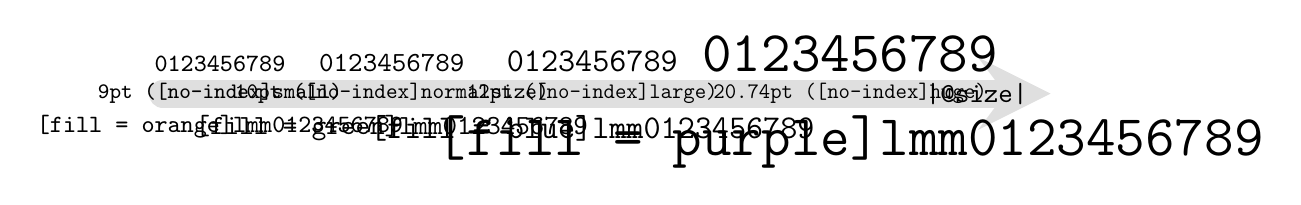
\begin{tikzpicture}[every node/.style = {font = \ttfamily}]
    \draw [ -stealth, gray!25, line width = 1em, line cap = round ]
      (0,0) --++ (.93\linewidth,0) node [ left, black ] {|\f@size|};
    \node [ above = 1ex ] at (.06\linewidth,0) {\small      0123456789};
    \node [ above = 1ex ] at (.24\linewidth,0) {\normalsize 0123456789};
    \node [ above = 1ex ] at (.45\linewidth,0) {\large      0123456789};
    \node [ above = 1ex ] at (.72\linewidth,0) {\huge       0123456789};
    \node [ below = 1ex ] at (.06\linewidth,0)
      {\small     \chartopath[fill = orange]{lmm}{0123456789}};
    \node [ below  = 1ex] at (.24\linewidth,0)
      {\normalsize\chartopath[fill = green]{lmm}{0123456789}};
    \node [ below = 1ex ] at (.45\linewidth,0)
      {\large     \chartopath[fill = blue]{lmm}{0123456789}};
    \node [ below = 1ex ] at (.72\linewidth,0)
      {\huge      \chartopath[fill = purple]{lmm}{0123456789}};
    \makeatletter
    \node at (.06\linewidth,0)
      {\small     \scalebox{\fpeval{8/\f@size}}
        {\small     \f@size pt (\cs[no-index]{small})}};
    \node at (.24\linewidth,0)
      {\normalsize\scalebox{\fpeval{8/\f@size}}
        {\normalsize\f@size pt (\cs[no-index]{normalsize})}};
    \node at (.45\linewidth,0)
      {\large     \scalebox{\fpeval{8/\f@size}}
        {\large     \f@size pt (\cs[no-index]{large})}};
    \node at (.72\linewidth,0)
      {\huge      \scalebox{\fpeval{8/\f@size}}
        {\huge      \f@size pt (\cs[no-index]{huge})}};
    \makeatother
  \end{tikzpicture}
\end{center}

\subsection{Use in \pkg{listings}}

This package can be used in the \pkg{listings} package, so that users could
directly copy and paste the source code from |.pdf| file without worry about
including unwanted line numbers.

\let\orithelstnumber\thelstnumber
  \def\thelstnumber{%
    \chartopath[fading = {red, violet, horizontal}]
      {lmm} {\orithelstnumber}%
  }
\begin{verbatim}
  \let\orithelstnumber\thelstnumber
  \def\thelstnumber{%
    \chartopath[fading = {red, violet, horizontal}]
      {lmm} {\orithelstnumber}%
  }
\end{verbatim}

\begin{example}
\begin{lstlisting}[language = {[LaTeX]TeX}]
\documentclass{article}
\begin{document}
  Hello, \LaTeX!
\end{document}
\end{lstlisting}
\end{example}

% % Test Indent???

% % \newbox\ttt
% % \sbox{\ttt}{\hbox{abc def}}
% % \showbox\ttt

% % \hskip1em 0123456789

%% \noindent\hskip2em
%% \chartopath[fill = teal] {lmm}\0

\section{Todo list}

\begin{itemize}
  \item [\textcolor{green}{\textsf{Detail}}] Baselines of several characters need to optimize.
  \item [\textcolor{red}{\textsf{Bug}}] Reading characters from a control sequence ("o-/e-"expand) \textcolor{red}{IS NOT STABLE!}.
  \item [\textcolor{red}{\textsf{Bug}}] Several special characters:
  Simplify user interface's input (problem of "rescan tokens").
  \item [\textcolor{blue}{\textsf{Function}}] Support function like
  "\chartopath{\usefont{T1}{cmr}{m}{sc} abc}", or\\
  "\chartopath{\sffamily abc}".
\end{itemize}

\end{documentation}

\begin{implementation}

\end{implementation}

% \PrintIndex

\end{document}
